\documentclass[12pt]{article}


\usepackage[dvips,letterpaper,margin=0.75in,bottom=0.75in]{geometry}
\usepackage{cite}
\usepackage{slashed}
\usepackage{graphicx}
\usepackage{amsmath}

\usepackage[american,fulldiode]{circuitikz}
\usetikzlibrary{calc}

\begin{document}
\ctikzset{bipoles/thickness=1}
\ctikzset{bipoles/length=.6cm}

\title{AM Radio}

\maketitle

\section{Introduction}

In this lab, you will build a fully operational AM radio receiver.  There are many ways to build an AM receiver.  The classic approach we use in this lab will highlight the key concepts we have encountered this quarter, including impedance, resonance, filtering, amplification, and negative feedback.  The AM radio is also an excellent introduction from every day life into the field of scientific instrumentation, which is generally aimed at extracting a small signal of interest in the presence of noise.

\begin{figure}[htbp]
\begin{center}
\begin{circuitikz}[american,line width=1pt]
\newcommand{\speaker}[2] % #1 = name from to[generic,n=#1], #2 = rotation angle
{\draw[thick, scale=0.5,line width=1pt,rotate=#2] (#1) +(.2,.25) -- +(.7,.75) -- +(.7,-.75) -- +(.2,-.25);}
\draw (0,0) node[buffer](rfamp){};
\draw (5,0) node[buffer](audioamp){};
\draw (rfamp.in) to[short] ++(-1.5,0) to[inductor,-*] ++(0,-1.5) node[ground,yscale=2.0]{} to[short] ++(0.75,0) to[vC,-*] ++(0,1.5);
\draw (rfamp.out) to[short] ++(0.5,0) to[D] ++(1.5,0) coordinate(X) to[short] (audioamp.in);
\draw (X) to[R,*-] ++(0,-1.5) to[short,-*] ++(0.75,0) node[ground,yscale=2.0]{} to[C,-*] ++(0,1.5);
\draw (audioamp.out) to[short] ++(0.5,0) to[generic,n=S] ++(0,-1.5) node[ground,yscale=2.0]{};
\speaker{S}{0}
\draw (-2,1.3) node[] {Tuner\vphantom{/p}};
\draw (0,1.3) node[] {RF Amp\vphantom{/p}};
\draw (2.5,1.3) node[] {Demodulator\vphantom{/p}};
\draw (6.0,1.3) node[] {Audio Filter/Amp\vphantom{/p}};
\end{circuitikz} 
\caption{Overview of the circuit we will be constructing.}
\label{fig:overview}
\end{center}
\end{figure}

An overview of the circuit we will be building is shown in Fig.~\ref{fig:overview}.  A large external antenna is inductively coupled to a resonant LC circuit.  By adjusting the value of the variable capacitor, the resonant frequency changes, and the AM radio station of interest is selected.  This weak radio frequency (RF) signal (of about 20~\rm mV) is amplified so that it is larger than a diode drop.  The signal is then demodulated by a diode plus low-pass filter, which is tuned to keep only the audio frequency (below $20~\rm kHz$).  The audio signal is than amplified and played on a speaker.

When working with anything complicated\footnote{Not just Electronics!} it is best to divide it into logical modules which can each be independently built and tested.  In this case, the instructor will provide the antenna and LC tuning circuit, simply because it is impractical to have 10 large antennas, but you should have a look at how it was built.  The instructor will also provide an audio power amplifier and speaker, based on the model you already built in the previous lab.  You are responsible for the RF amplifier, the Demodulator, and the Audio filter.

Getting this all to work in one lab session will be a challenge.  For that reason, a progressive grading scale will be used (i.e. you will get nearly full credit even if you don't get to the end.)

You will need to move your board to test it, so make certain to use the voltage plug-in sockets at the top of your board to power and ground it.  Keep it neat and color coded... you won't be allowed to plug into the antenna and audio system unless it is a neat and orderly circuit! 

\section{Demodulation Stage}

\begin{figure}[htbp]
\begin{center}
\begin{circuitikz}[american,line width=1pt]
\draw (0,0) node[left]{$v_{\rm in}$}  to[C,l=$C_1$,-*] ++(1.5,0) coordinate(X);
\draw (X) to[R,l=$R_1$] ++(0,-1.5) node[ground,yscale=2.0]{};
\draw (X) to[D,l=D] ++(1.5,0) coordinate(Y) to[short,*-o] ++(2.5,0) node[right]{$v_{\rm out}$};
\draw (Y) to[R,l=$R_2$] ++(0,-1.5) to[short,-*] ++(1.5,0) node[ground,yscale=2.0]{} to[C,l_=$C_2$,-*] ++(0,1.5);
\end{circuitikz} 
\caption{A passive AM demodulator.}
\label{fig:demod}
\end{center}
\end{figure}

Build the circuit in Fig.~\ref{fig:demod} using a 1N914 switching diode with $R_1 = R_2 = 120~\rm k\Omega$, $C_1=10~\rm nF$, and $C_2=470~\rm pF$.   For testing purposes, drive the input with a $1~\rm MHz$ sine wave with $5~\rm V$ peak-to-peak voltage.   And view the input and output simultaneously on your scope, taking care that both channels are DC biased.  It is instructive to view the output first without the capacitor $C_2$, so that you can observe the diode rectifying the $1~\rm MHz$ signal.  Then insert $C_2$ back into your circuit and observe that the output, which should now be a nearly constant value, which is non-zero due to the rectification.

Next, learn how to use your function generator's modulation function to modulate the $5~\rm V$ at $1~\rm MHz$ sine wave by an audio tone of $900~\rm Hz$.  You should now see the input signal bouncing around at $1~\rm MHz$ but if you trigger on the output (and stop viewing the input) you will observe your reconstructed audio signal.  Note that you will have to change the time-scale from $1~\rm MHz$ range to $1~\rm kHz$ range!
Once you have a clear demodulated audio signal, note the distortion due to the diode drop in our passive rectifier:  there will be a flat section of your sine wave.  Confirm that if you adjust your AM frequency, your reconstructed audio signal also changes.  Your demodulation stage is complete!

\section{RF Amplifier}

\begin{figure}[htbp]
\begin{center}
\begin{tabular}{c@{\hskip 2cm}c}
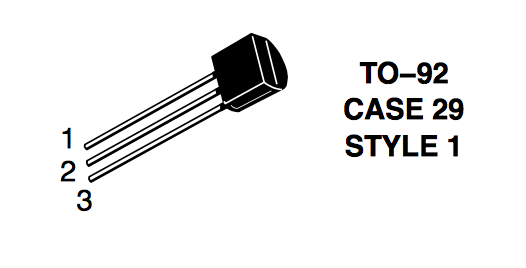
\includegraphics[height=0.10\textheight]{figs/case3904.png} &
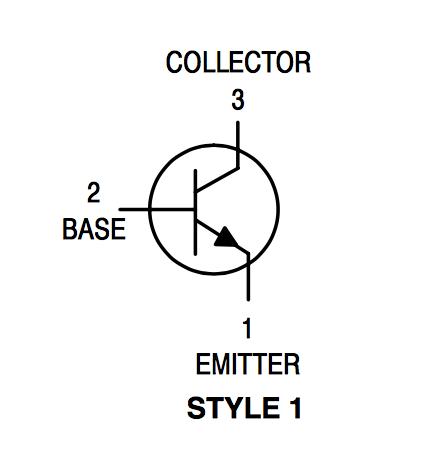
\includegraphics[height=0.18\textheight]{figs/chan3904.png} \\
\end{tabular}
\end{center}
\caption{The TO-92 Style 1 package used for some discrete transistors, including the 2N5088 transistor used throughout this lab.  Note that not all transistors use the same pinout, even if they are in the TO-92 package.}
\label{fig:layout}
\end{figure}

In this section your are going to build the RF amplifier circuit shown in Fig.~\ref{fig:rfamp}.  I suggest you build this in stages:  (1) build only the DC-biasing voltage divider ($R_1$, $R_2$, and $R_3$) and check that DC bias points, (2) connect the transistors and the resistors ($R_4$, $R_5$, $R_6$) and the capacitor $C_3$, check the DC bias points, and confirm there is a diode drop across the base and emitter at each transistor, (3) connect the capacitors $C_1$ and $C_2$.  

You will use special high-beta 2N5088 transistors, and $R_1=390~\rm k\Omega$, $R_2=22~\rm k\Omega$, $R_3=47~\rm k\Omega$, $R_4=12~\rm k\Omega$, $R_5=220~\rm \Omega$, $R_6=1~\rm k\Omega$, $C_1=C_2=10~\rm nF$ and $C_3=1~\rm nF$.   Use your bench-top DC power-supply to provide $V_{\rm cc} = 10~\rm V$ and $V_{\rm EE}= -10~\rm V$.   When using dual supplies, remember that your bench-top DC supply is not ground referenced, so you must explicitly connect the ground as well.


Return your function generator to continuous (no modulation) mode.  Measure the gain for an input signal of $100~\rm mV$ at a frequency of $1~\rm MHz$ (you should see about $G \sim 20$).

Now build and test a second copy of the circuit in Fig.~\ref{fig:rfamp}.

When both stages are working, gang them together, and check the combined gain.

\section{Testing}

Now connect the two RF amplifier to your demodulation circuit, and confirm that you can now demodulate an AM signal with amplitude of only $20~\rm mV$.  You are ready to test your circuit with the antenna and audio system.  Put your name on the waiting list after your circuit is checked for clarity and neatness. 





\begin{figure}[htbp]
\begin{center}
\begin{circuitikz}[american,line width=1pt]
\draw (0,0) node[npn](npn1){};
\draw ++(0,2) node[npn](npn2){}; 
\draw (npn2.E) to[short] (npn1.C);
\draw (npn2.C) to[short,*-o] ++(0.5,0) node[right]{$v_{\rm out}$};
\draw (npn2.C) to[R,l=$R_4$,-*] ++(0,1.5) coordinate(X) to[short,*-o] ++(0,0.5) node[right]{$V_{\rm CC}$};
\draw (X) to[short] ++(-3.0,0) to[R,l_=$R_1$] ++(0,-1.5) coordinate(X);
\draw let \p1 = (npn2.B), \p2=(X) in coordinate(Y) at (\x2,\y1);
\draw (X) to[short] (Y) coordinate(X);
\draw (npn2.B) to[short,-*] (X) to[C,l=$C_1$] ++(-1.5,0) node[ground,yscale=2.0]{};
\draw let \p1 = (npn1.B), \p2=(X) in coordinate(Y) at (\x2,\y1);
\draw (X) to[R,l=$R_2$] (Y)  coordinate(X);
\path (X) ++ (1.5,0) coordinate(A);
\draw (A) to[short] (npn1.B);
\draw (A) to[short,-*] (X) to[C,l=$C_2$,-o] ++(-1.5,0) node[left]{$v_{\rm in}$};
\draw let \p1 = (npn1.E), \p2=(X) in coordinate(Y) at (\x2,\y1);
\draw (X) to[short] (Y) to[R,l_=$R_3$] ++(0,-1.5) coordinate(C);
\draw (npn1.E) to[R,l=$R_5$] ++(0,-1.5) coordinate(X) to[R,l=$R_6$,-*] ++(0,-1.5) coordinate(Y) to[short,*-o] ++(0,-0.5) node[right]{$V_{\rm EE}$};
\draw (Y) -| (C);
\draw (X) to[short,*-] ++(-1.0,0) to[C,l_=$C_3$,-*] ++(0,-1.5);
%(A) to[R,l=$R_4$,*-*] ++(0,-1.5) coordinate(B)
%let \p1 = (npn1.E), \p2=(B) in coordinate(C) at (\x1,\y2)
%(B) to[C,l_=$C_3$,-*] (C) to[short] (npn1.E)
%let \p1 = (B), \p2=(X) in coordinate(Y) at (\x2,\y1)
%(B) to[short,-*] (Y)
%(C) to[R,l=$R_6$] ++(0,-1.5) coordinate(D) to[R,l=$R_7$,-*] ++(0,-1.5) coordinate(E) node[ground,yscale=2.0]{} 
%(X) |- (E)
%(D) to[short,*-] ++(-1.5,0) to[C,l_=$C_4$,-*] ++(0,-1.5)
\end{circuitikz} 
\caption{RF amplifier featuring a cascode and an emitter-resistor bypass capacitor.}
\label{fig:rfamp}
\end{center}
\end{figure}


\begin{figure}[htbp]
\begin{center}
\begin{tabular}{c@{\hskip 2cm}c}
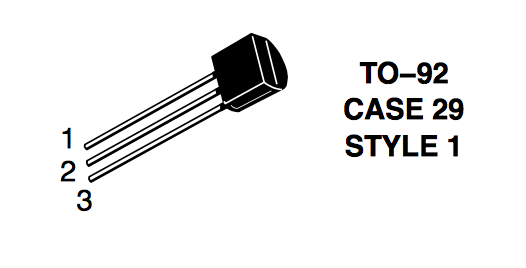
\includegraphics[height=0.10\textheight]{figs/case3904.png} &
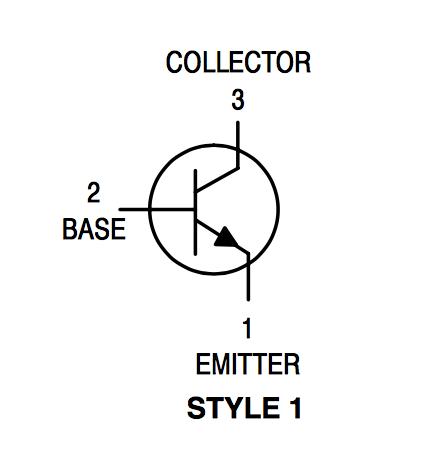
\includegraphics[height=0.18\textheight]{figs/chan3904.png} \\
\end{tabular}
\end{center}
\caption{The TO-92 Style 1 package used for some discrete transistors, including the 2N5088 transistor used throughout this lab.  Note that not all transistors use the same pinout, even if they are in the TO-92 package.}
\label{fig:layout}
\end{figure}

\begin{figure}[htbp]
\begin{center}
\includegraphics[height=0.50\textheight]{figs/first_finished.jpg} 
\end{center}
\caption{The first student circuit to finish succesfully.  Neat work is fast work!}
\label{fig:layout}
\end{figure}


\section{Lab Report}
There is no lab report needed for this assignment. 







\end{document}
